% Setup appearance:
\documentclass{beamer}
%\usetheme{Darmstadt}
\usefonttheme[onlylarge]{structurebold}
\setbeamerfont*{frametitle}{size=\normalsize,series=\bfseries}
\setbeamertemplate{navigation symbols}{}


% Standard packages

\usepackage[english]{babel}
\usepackage[latin1]{inputenc}
\usepackage{times}
\usepackage[T1]{fontenc}
\usepackage{makeidx} % allows for indexgeneration
\usepackage{graphicx}
\usepackage{multicol}
\usepackage{subfigure}
\usepackage{mathptmx} % use Times fonts if available on your TeX system
\usepackage{setspace}
\usepackage{epsfig}
% Setup TikZ
\usepackage{tikz}
\usetikzlibrary{arrows}
\tikzstyle{block}=[draw opacity=0.7,line width=1.4cm]


% Author, Title, etc.

\title[Robotic Validation of AFM and Beyond] 
{%
  Robotic Validation of AFM, Scale-freeness, Local Communication etc.%
}

\author[MOFSarker]
{
  Md Omar Faruque Sarker
}

\institute[UWN]
{
 Robotic Intelligence Lab\\
 University of Wales, Newport
}

\date{May 2010}



% The main document

\begin{document}

\begin{frame}
  \titlepage
\end{frame}

\begin{frame}{Outline}
  \tableofcontents
\end{frame}


\section{Introduction}

\subsection{Update since last meeting in Dec 2009}

\begin{frame}{Software code, experiments, papers, Hardware up-gradation ...}
  \begin{itemize}
    \item \alert{Software code on {\em HEAD}}\\
     \hspace*{2mm} Hybrid Event-Driven Architecture on D-Bus
    \item  \alert{AFM validation experiments:}\\
     \hspace*{2mm} using centralized and local communication\\
      \hspace*{2mm} (approx. 15 hours, with 8 and 16 robots)
    \item \alert{Three conference papers:}\\
     \hspace*{2mm} - ANTS 2010 (Belgium): {\em accepted}\\
     \hspace*{2mm} - IROS 2010 (Taiwan)\\
     \hspace*{2mm} - Control 2010 (UK) 
    \item \alert{Extending robot hardware:}\\  
     \hspace*{2mm}Bluetooth $\rightarrow$ Wifi for 16 to 40 robots
    \item \alert{Only 3-4 months left:} to wrap-up everything..:-)
    \end{itemize}
\end{frame}
%%%%%%%%%%%%%%%%%%%%%%%%%%
\subsection{Short review  }
\begin{frame}[t]{What is self-organization... ?}
\begin{figure}
\centering
\includegraphics[height=6cm, angle=0]
{/media/Preload/Pub2010/ThoughtsLinedUp/images/dia-files/self-org-1}
%figure caption is below the figur
\caption{\small The 4 perspectives}
\label{fig:afm} % Give a unique label
\end{figure}
\end{frame}

\begin{frame}[t]{Self-regulation of an agent}  
\begin{figure}
\centering
\includegraphics[height=4cm, angle=0]
{/media/Preload/Pub2010/ThoughtsLinedUp/images/dia-files/self-org-agent}
%\caption{\small Agent's self-regulation} % for implementing AFM}
\label{fig:setup} % Give a unique label
\end{figure}
\end{frame}


%%%%%%%%%%%%%%%%%%%%%%%%%%%%%
\begin{frame}[t]{So, AFM: \alert{the 4 stars} in sky of self-organization?}  
\begin{figure}
\centering
\includegraphics[height=5cm, angle=0]
{/media/Preload/Pub2010/ThoughtsLinedUp/images/dia-files/self-org-2}
%figure caption is below the figure
%\caption{\small }
\label{fig:setup} % Give a unique label
\end{figure}
\end{frame}

%\begin{frame}[t]{From AFM:}
% \begin{block}{Key mechanisms for self-regulation? }
%    \begin{itemize}
%    \item Presence of continuous flow of information
%    \item Concurrency of tasks: multiple tasks simultaneously 
%    \item Learning: key to specialization
%    \item Forgetting: key to flexibility
%    \end{itemize}
%  \end{block}
%\end{frame}

\section{Robotic Validation of AFM}

\subsection{Centralized Communication Mode - Global attractive filed sensing and no P2P communication}

\begin{frame}[t]{Robotic Validation of AFM}
\begin{figure}
\centering
\includegraphics[height=5cm, angle=0]
{/media/Preload/Pub2010/ANTS2010-Draft/dia-files/RIL-Expt-Setup2}
%figure caption is below the figure
%\caption{\small }
\label{fig:setup} % Give a unique label
\end{figure}
 \begin{block}{Robots, Tasks, Camera, Bluetooth and \alert{beep beep beep...} }
 \begin{scriptsize}
    \begin{itemize}
    \item 5 x Centralized comm. expt: 8 robots/2 tasks/ 2 sq. m. (~60min)
    \item 5 x Centralized comm. expt: 16 robots/ 4 tasks / 4 sq. m. (~40min)
    \item 3 x Local comm. mode expt : 16 robots, 1m radii of comm. (~40min)
    \item 3 x Local comm. mode expt : 0.5m radii of comm. (~40min)
    \end{itemize}
 \end{scriptsize}
  \end{block}
\end{frame}

\begin{frame}[t]{Virtual Manufacturing Shop-floor: \alert{TODO of Future}}
\begin{figure}
\centering
\includegraphics[height=7cm, angle=0]
{/media/Preload/Pub2010/ANTS2010-Draft/dia-files/VSP}
%figure caption is below the figure
%\caption{\small }
\label{fig:setup} % Give a unique label
\end{figure}
\end{frame}

\begin{frame}[t]{Experimental Parameters: \alert{Size doesn't matter}}
\begin{table}
%\caption{Experimental parameters}
\label{table:params}
\begin{small}
\begin{center}
\begin{tabular}{|l||c|}
\hline Parameter & Value\\
\hline Total number of robots ($N$) & 16\\
\hline Total number of tasks ($M$) & 4\\
\hline Experiment area ($A$) & 4 $m^2$\\
\hline Initial production work-load/machine ($\Omega_{j}^{p}$) & 100 unit\\
\hline Task urgency increase rate ($\Delta\phi_{INC}$) & 0.005\\
\hline Task urgency decrease rate ($\Delta\phi_{DEC}$) & 0.0025\\
\hline Initial sensitization ($K_{INIT}$) & 0.1\\
\hline Sensitization increase rate ($\Delta k_{INC}$) & 0.03\\
\hline Sensitization decrease rate ($\Delta k_{DEC}$) & 0.01\\
%\hline A very small distance ($\delta$)& 0.000001\\
\hline Task info update interval ($\Delta TS_{u}$) & 5s\\
%\hline Task info signal emission interval ($ \Delta TS_{e}$)& 2.5s\\
%\hline Robot's task time-out interval ($\Delta RT_{to} $)& 10s\\
\hline
\end{tabular}
\end{center}
\end{small}
\end{table}
\end{frame}
%%
%%% Results
\begin{frame}[t]{Snapshot of Task Urgencies: \alert{Call for duty..}}
\begin{figure}
\centering
\includegraphics[height=7cm, angle=0]
{/media/Preload/Pub2010/ANTS2010-Draft/draft/images/PlotUrgencyLog-2010May10-115549}
%figure caption is below the figure
%\caption{\small }
\label{fig:setup} % Give a unique label
\end{figure}
\end{frame}
%%
\begin{frame}[t]{Workload: \alert{I'm free to wander or work...}}
\begin{figure}
\centering
\includegraphics[height=7cm, angle=0]
{/media/Preload/Pub2010/ANTS2010-Draft/draft/images/TaskUrgencyStat}
%figure caption is below the figure
%\caption{\small }
\label{fig:setup} % Give a unique label
\end{figure}
\end{frame}
%%
\begin{frame}[t]{Workers: \alert{Ready to serve in your need}}
\begin{figure}
\centering
\includegraphics[height=7cm, angle=0]
{/media/Preload/Pub2010/ANTS2010-Draft/draft/images/WorkerRatio}
%figure caption is below the figure
%\caption{\small }
\label{fig:setup} % Give a unique label
\end{figure}
\end{frame}
%
\begin{frame}[t]{Global attractive filed: \alert{that made us crazy}}
\begin{figure}
\centering
\includegraphics[height=7cm, angle=0]
{/media/Preload/Pub2010/ANTS2010-Draft/draft/images/global/Global-SignalingFreqStat}
%figure caption is below the figure
%\caption{\small }
\label{fig:setup} % Give a unique label
\end{figure}
\end{frame}
%%
\begin{frame}[t]{Who did the work: \alert{Oh! yes some of us...}}
\begin{figure}
\centering
\includegraphics[height=7cm, angle=0]
{/media/Preload/Pub2010/ANTS2010-Draft/draft/images/TaskSpecialization-task3-10may-1}
%figure caption is below the figure
%\caption{\small }
\label{fig:setup} % Give a unique label
\end{figure}
\end{frame}
%%
\begin{frame}[t]{Forget about everything: \alert{we need some rest}}
\begin{figure}
\centering
\includegraphics[height=7cm, angle=0]
{/media/Preload/Pub2010/ANTS2010-Draft/draft/images/global/RobotSensitizationStat-Total-50steps}
%figure caption is below the figure
%\caption{\small }
\label{fig:setup} % Give a unique label
\end{figure}
\end{frame}
%%
%%%%%%%%%%%%
\section{Local P2P Communication Model}
\subsection{Local  attractive filed sensing and local P2P communication }

\begin{frame}[t]{Local sensing/comm.: \alert{Talk less, Move less, Work more}}
\begin{figure}
\centering
\begin{tabular}{cc}
\epsfig{file=/media/Preload/Pub2010/ANTS2010-Draft/draft/images/global/Global-SignalingFreqStat.eps,width=0.48\linewidth,clip=} &
\epsfig{file=/media/Preload/Pub2010/ANTS2010-Draft/draft/images/global/DeltaTranslationStat.eps,width=0.48\linewidth,clip=} \\
\epsfig{file=/media/Preload/Pub2010/ANTS2010-Draft/draft/images/local-500cm/Local-500cm-SignalingFreqStat.eps,width=0.5\linewidth,clip=} &
\epsfig{file=/media/Preload/Pub2010/ANTS2010-Draft/draft/images/local-500cm/DeltaTranslationStat.eps,width=0.41\linewidth,clip=}
\end{tabular}
\end{figure}
\end{frame}


\section{Next: Scale-freeness, Random communication}
\subsection{Keeping the ratios of robots, tasks, area etc. constant}
\begin{frame}[t]{Next: \alert{sky is the limit...}}

 \begin{block}{Hardware upgrade, More experiments, publishing ... }
    \begin{itemize}
    \item Local communication with \alert{random peer selection}
    \item Scale-freeness: \alert{Compare 4 sets of expt: 40, 32, 16, 8 robots}
    \item Virtual Shop-floor $\Leftarrow$ \alert{real-task implementation} etc.
    \end{itemize}
  \end{block}
\begin{figure}
\centering
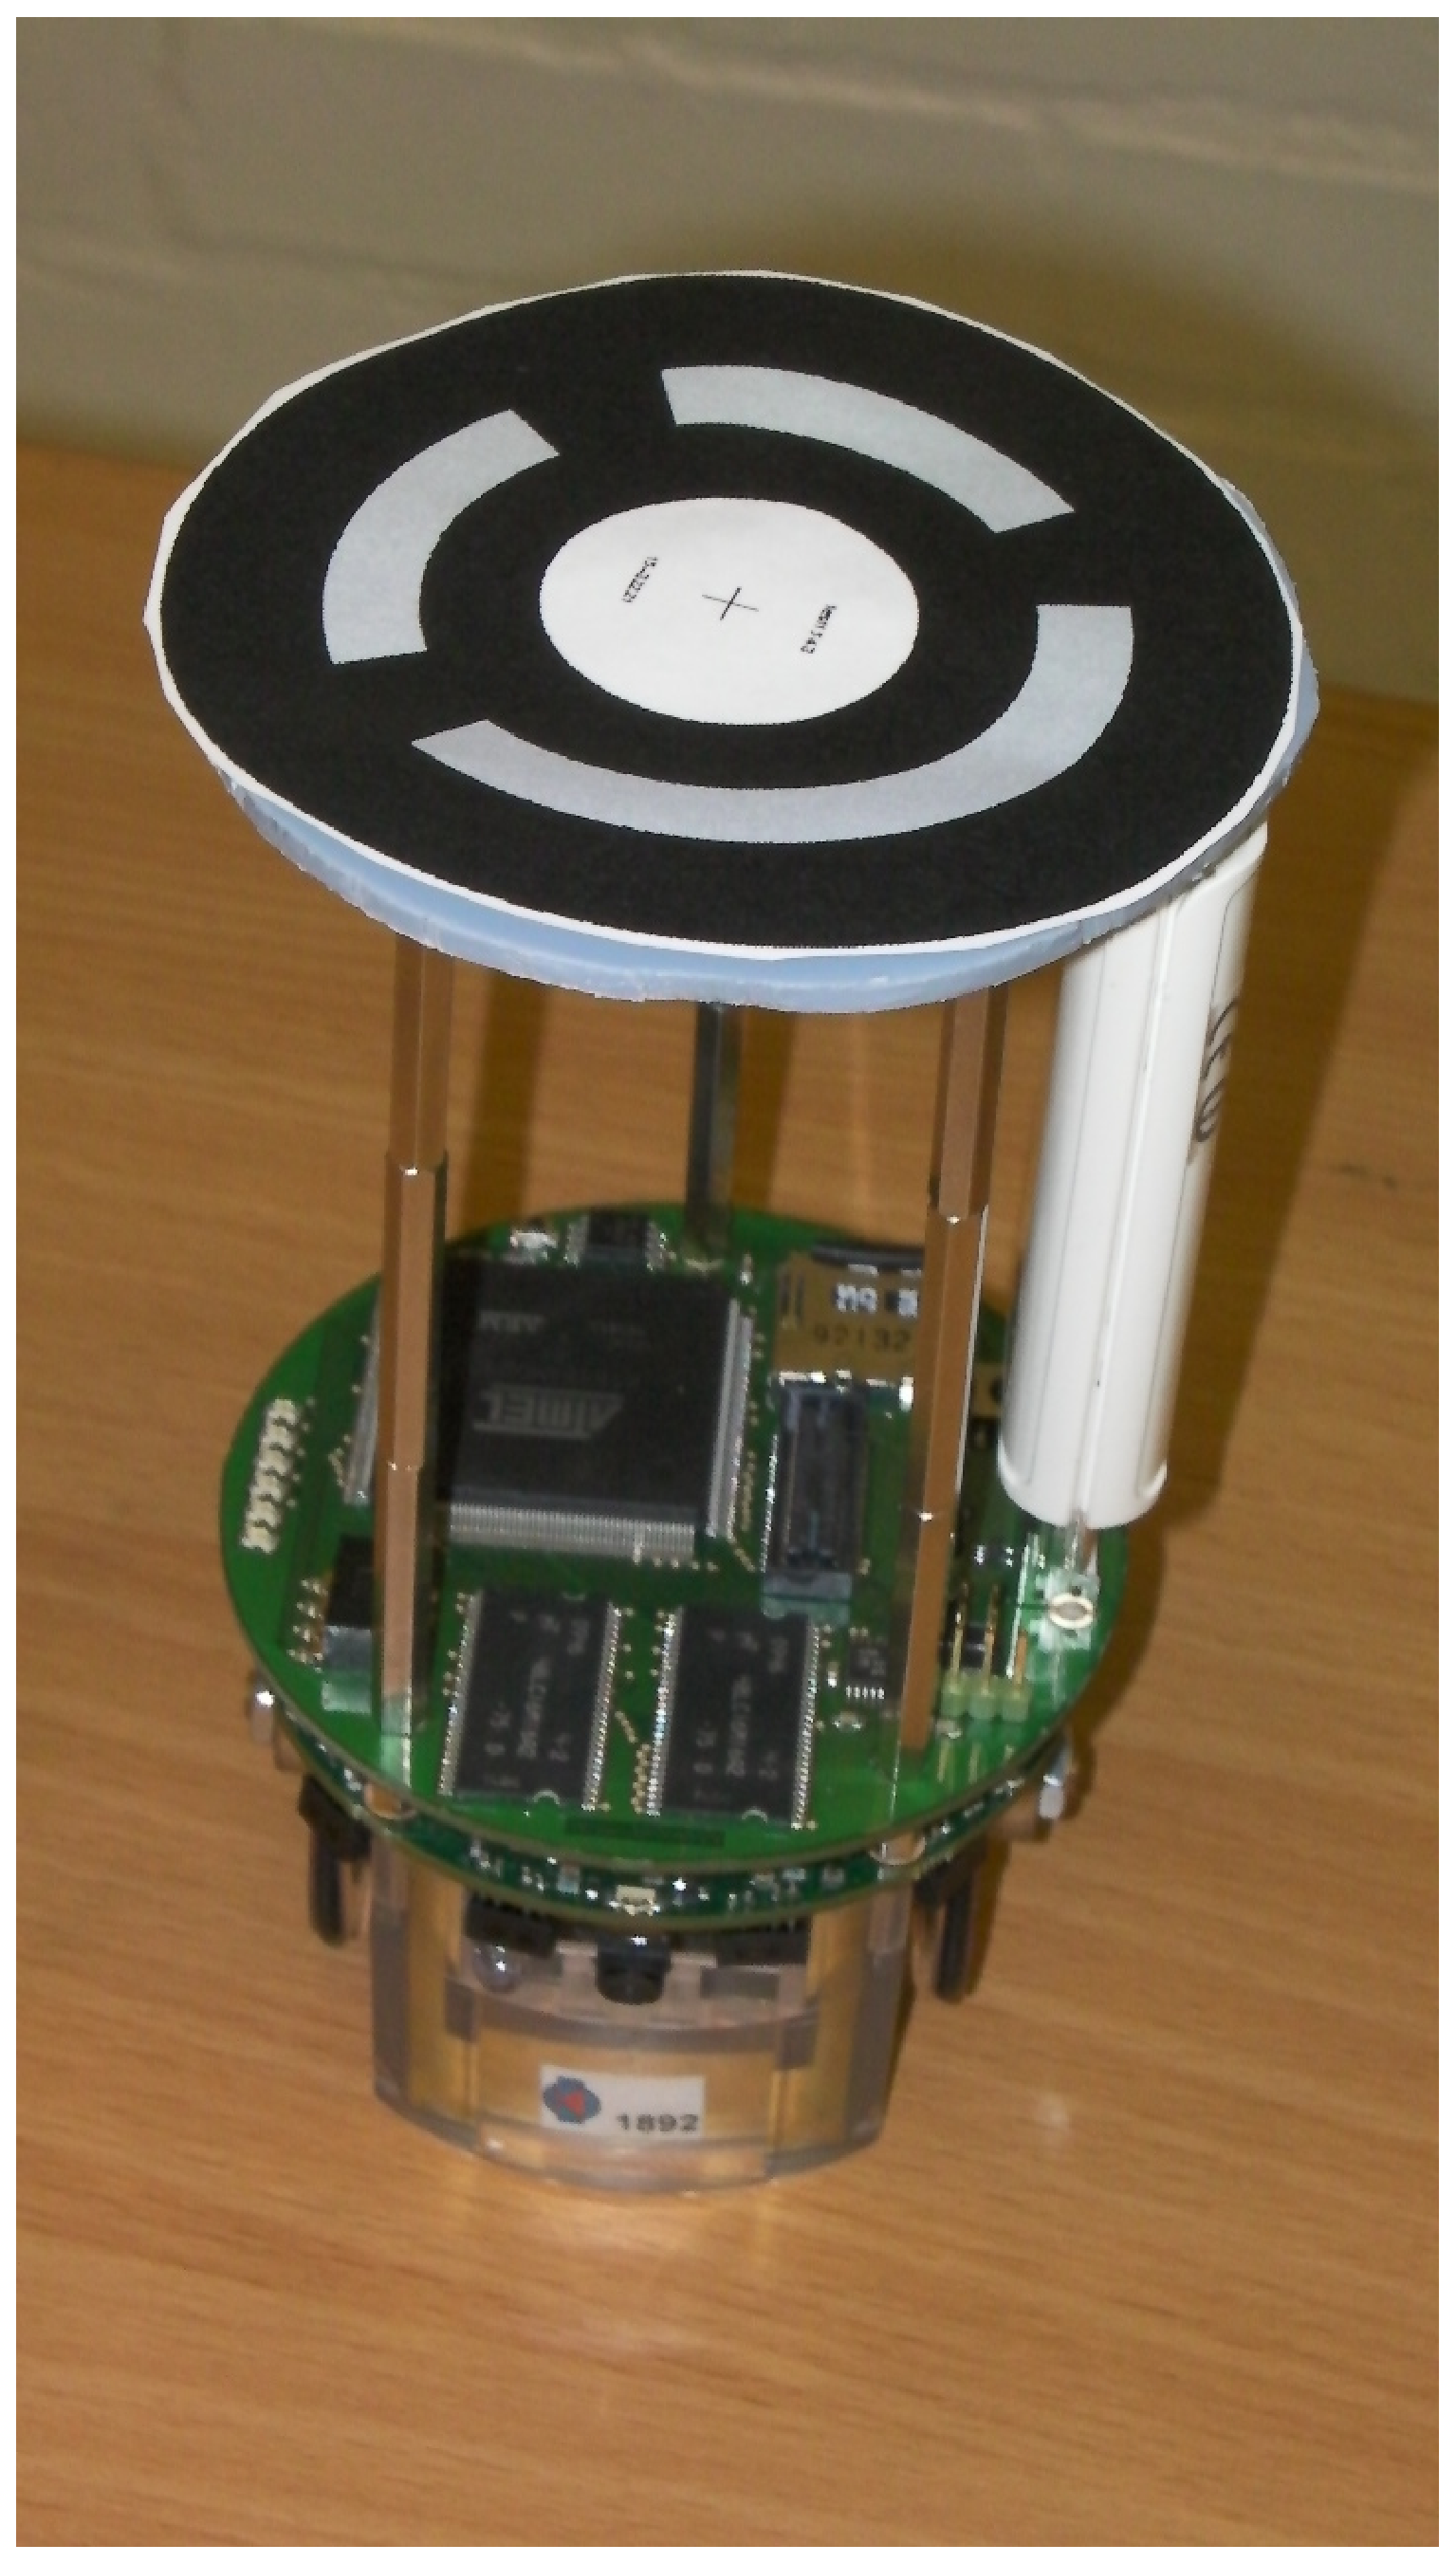
\includegraphics[height=4cm, angle=0]{epuck-linux-port}
\caption{\scriptsize New Epuck robot with Wifi and Linux extension board}
\end{figure}
\end{frame}

\begin{frame}[t]{32 robots in action: \alert{Camera ready, blind closed ..}}
\begin{figure}
\centering
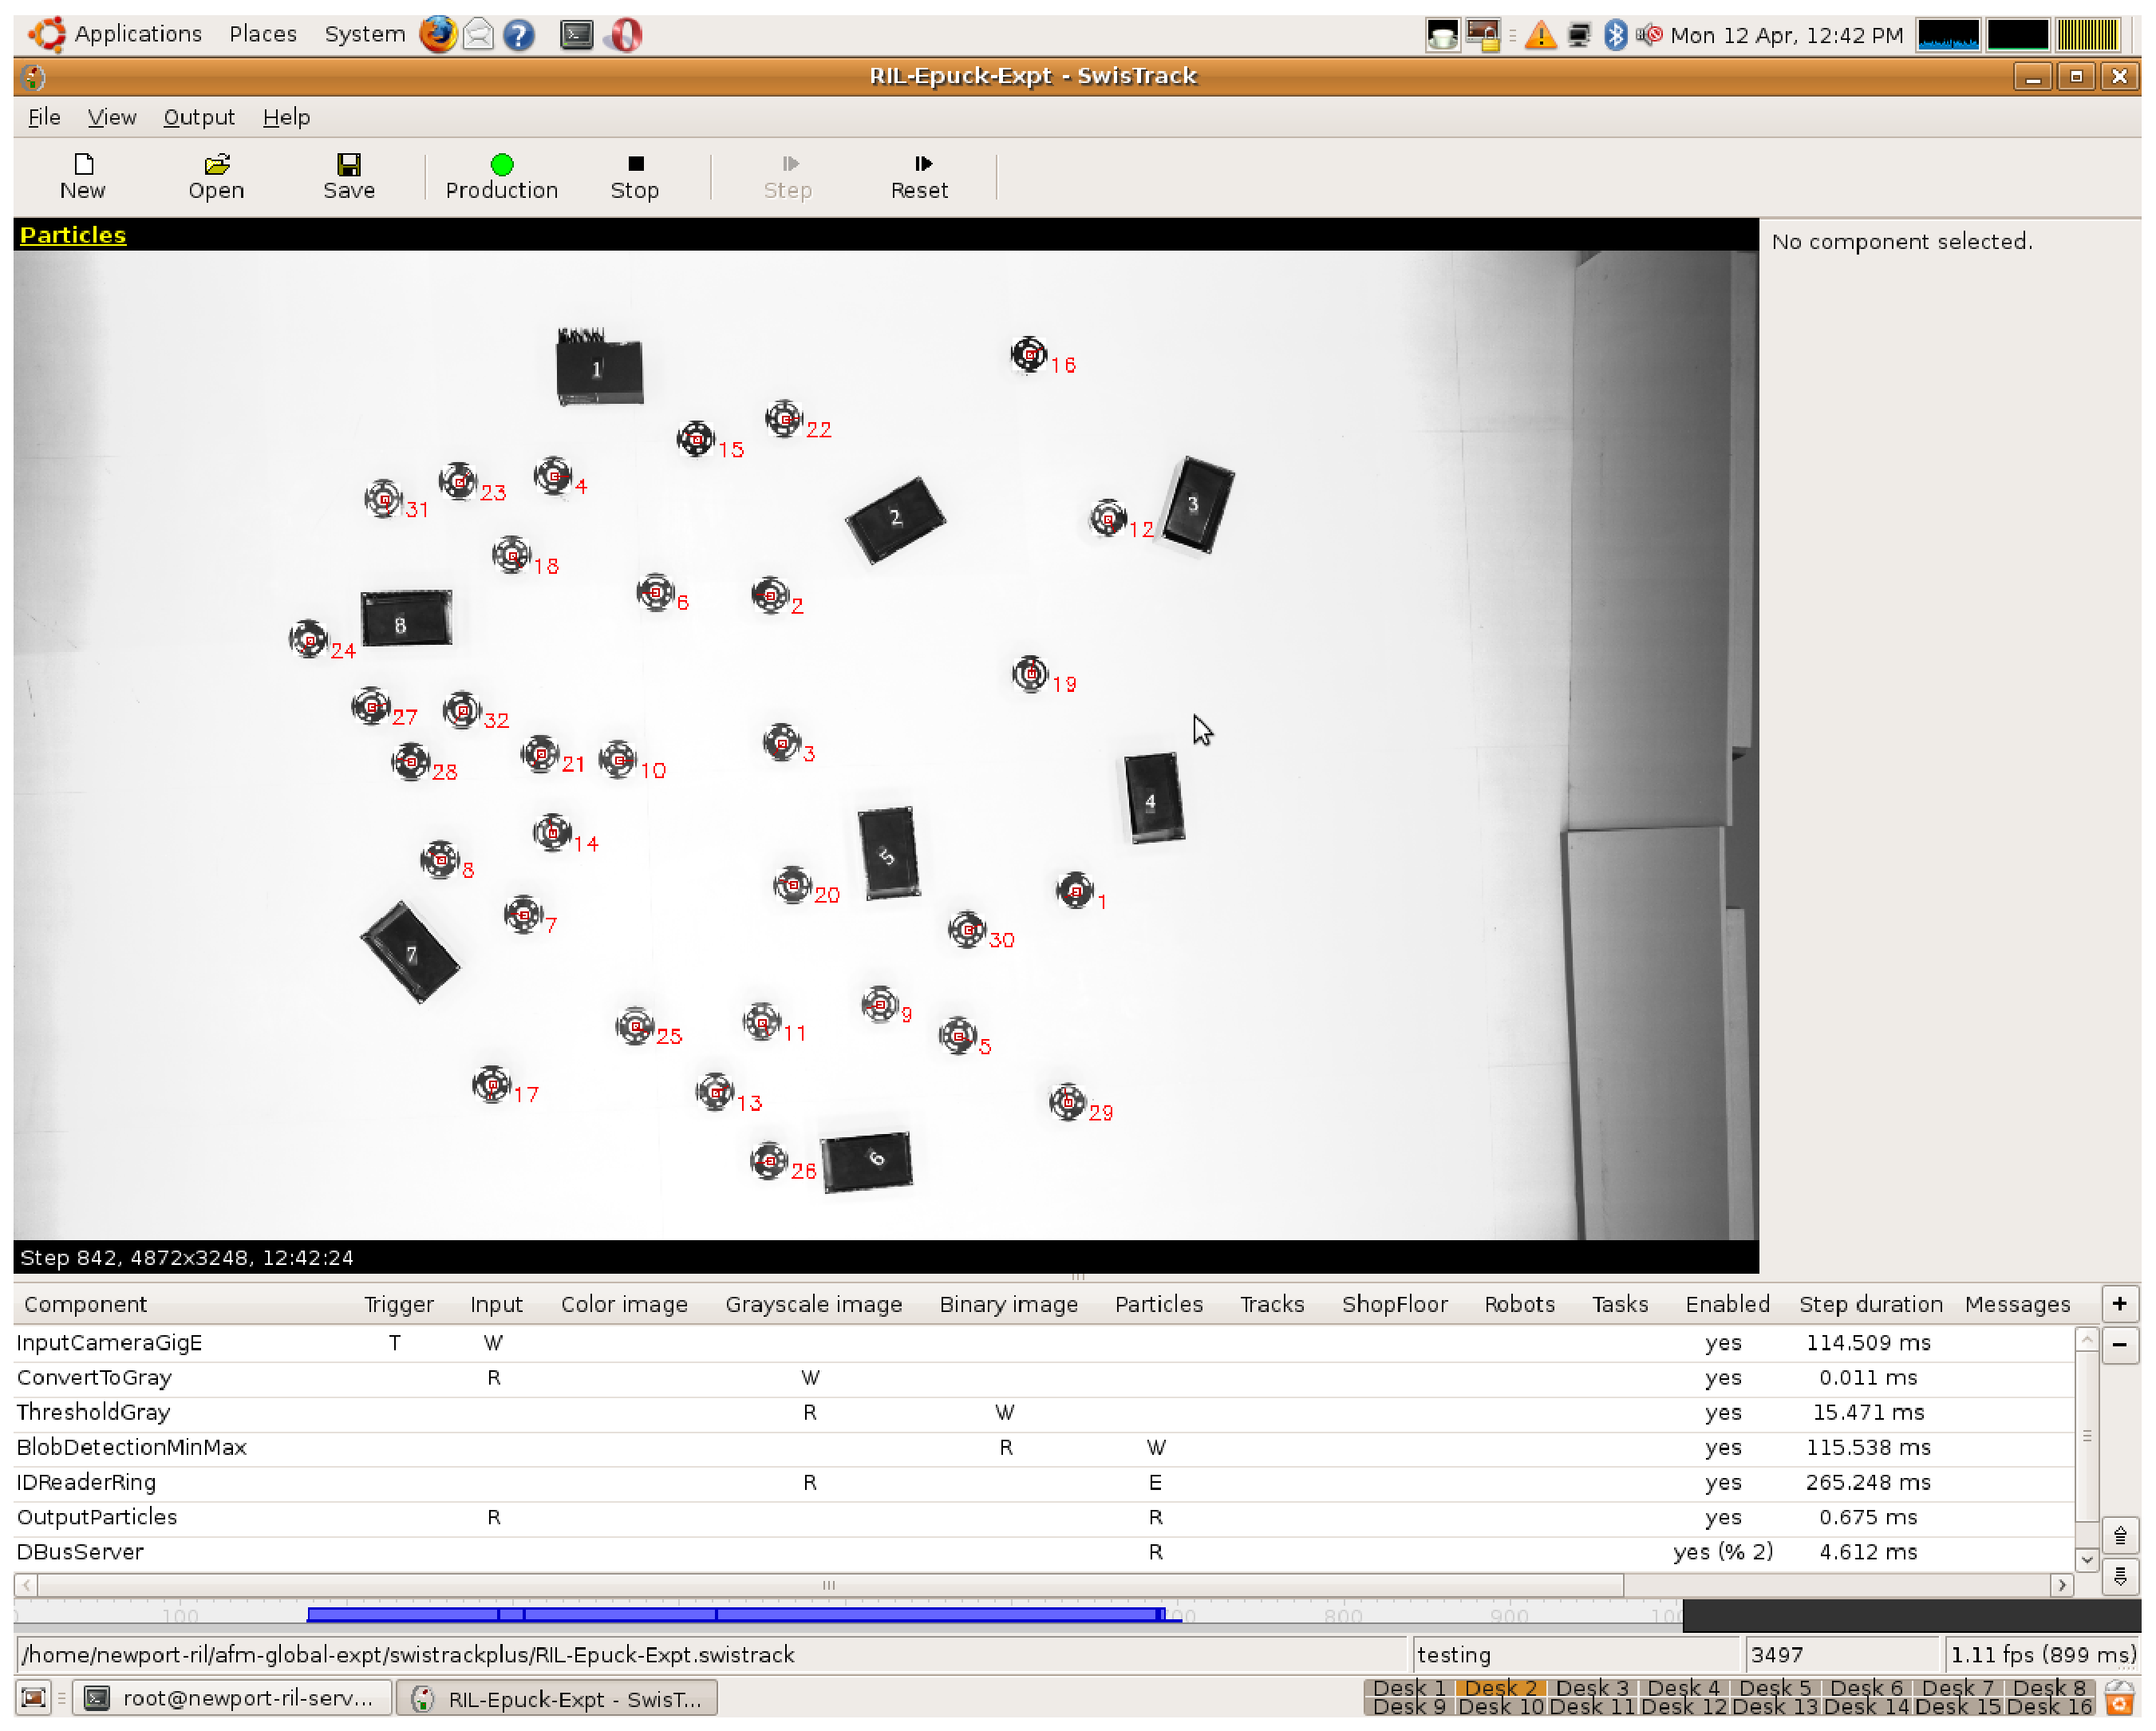
\epsfig{file=Screenshot-32markers-8tasks.eps,width=0.8\linewidth,clip=}
\end{figure}
\end{frame}

\begin{frame}[t]{Tracking all 40 robots: \alert{Camera ready, light up ..}}
\begin{figure}
\centering
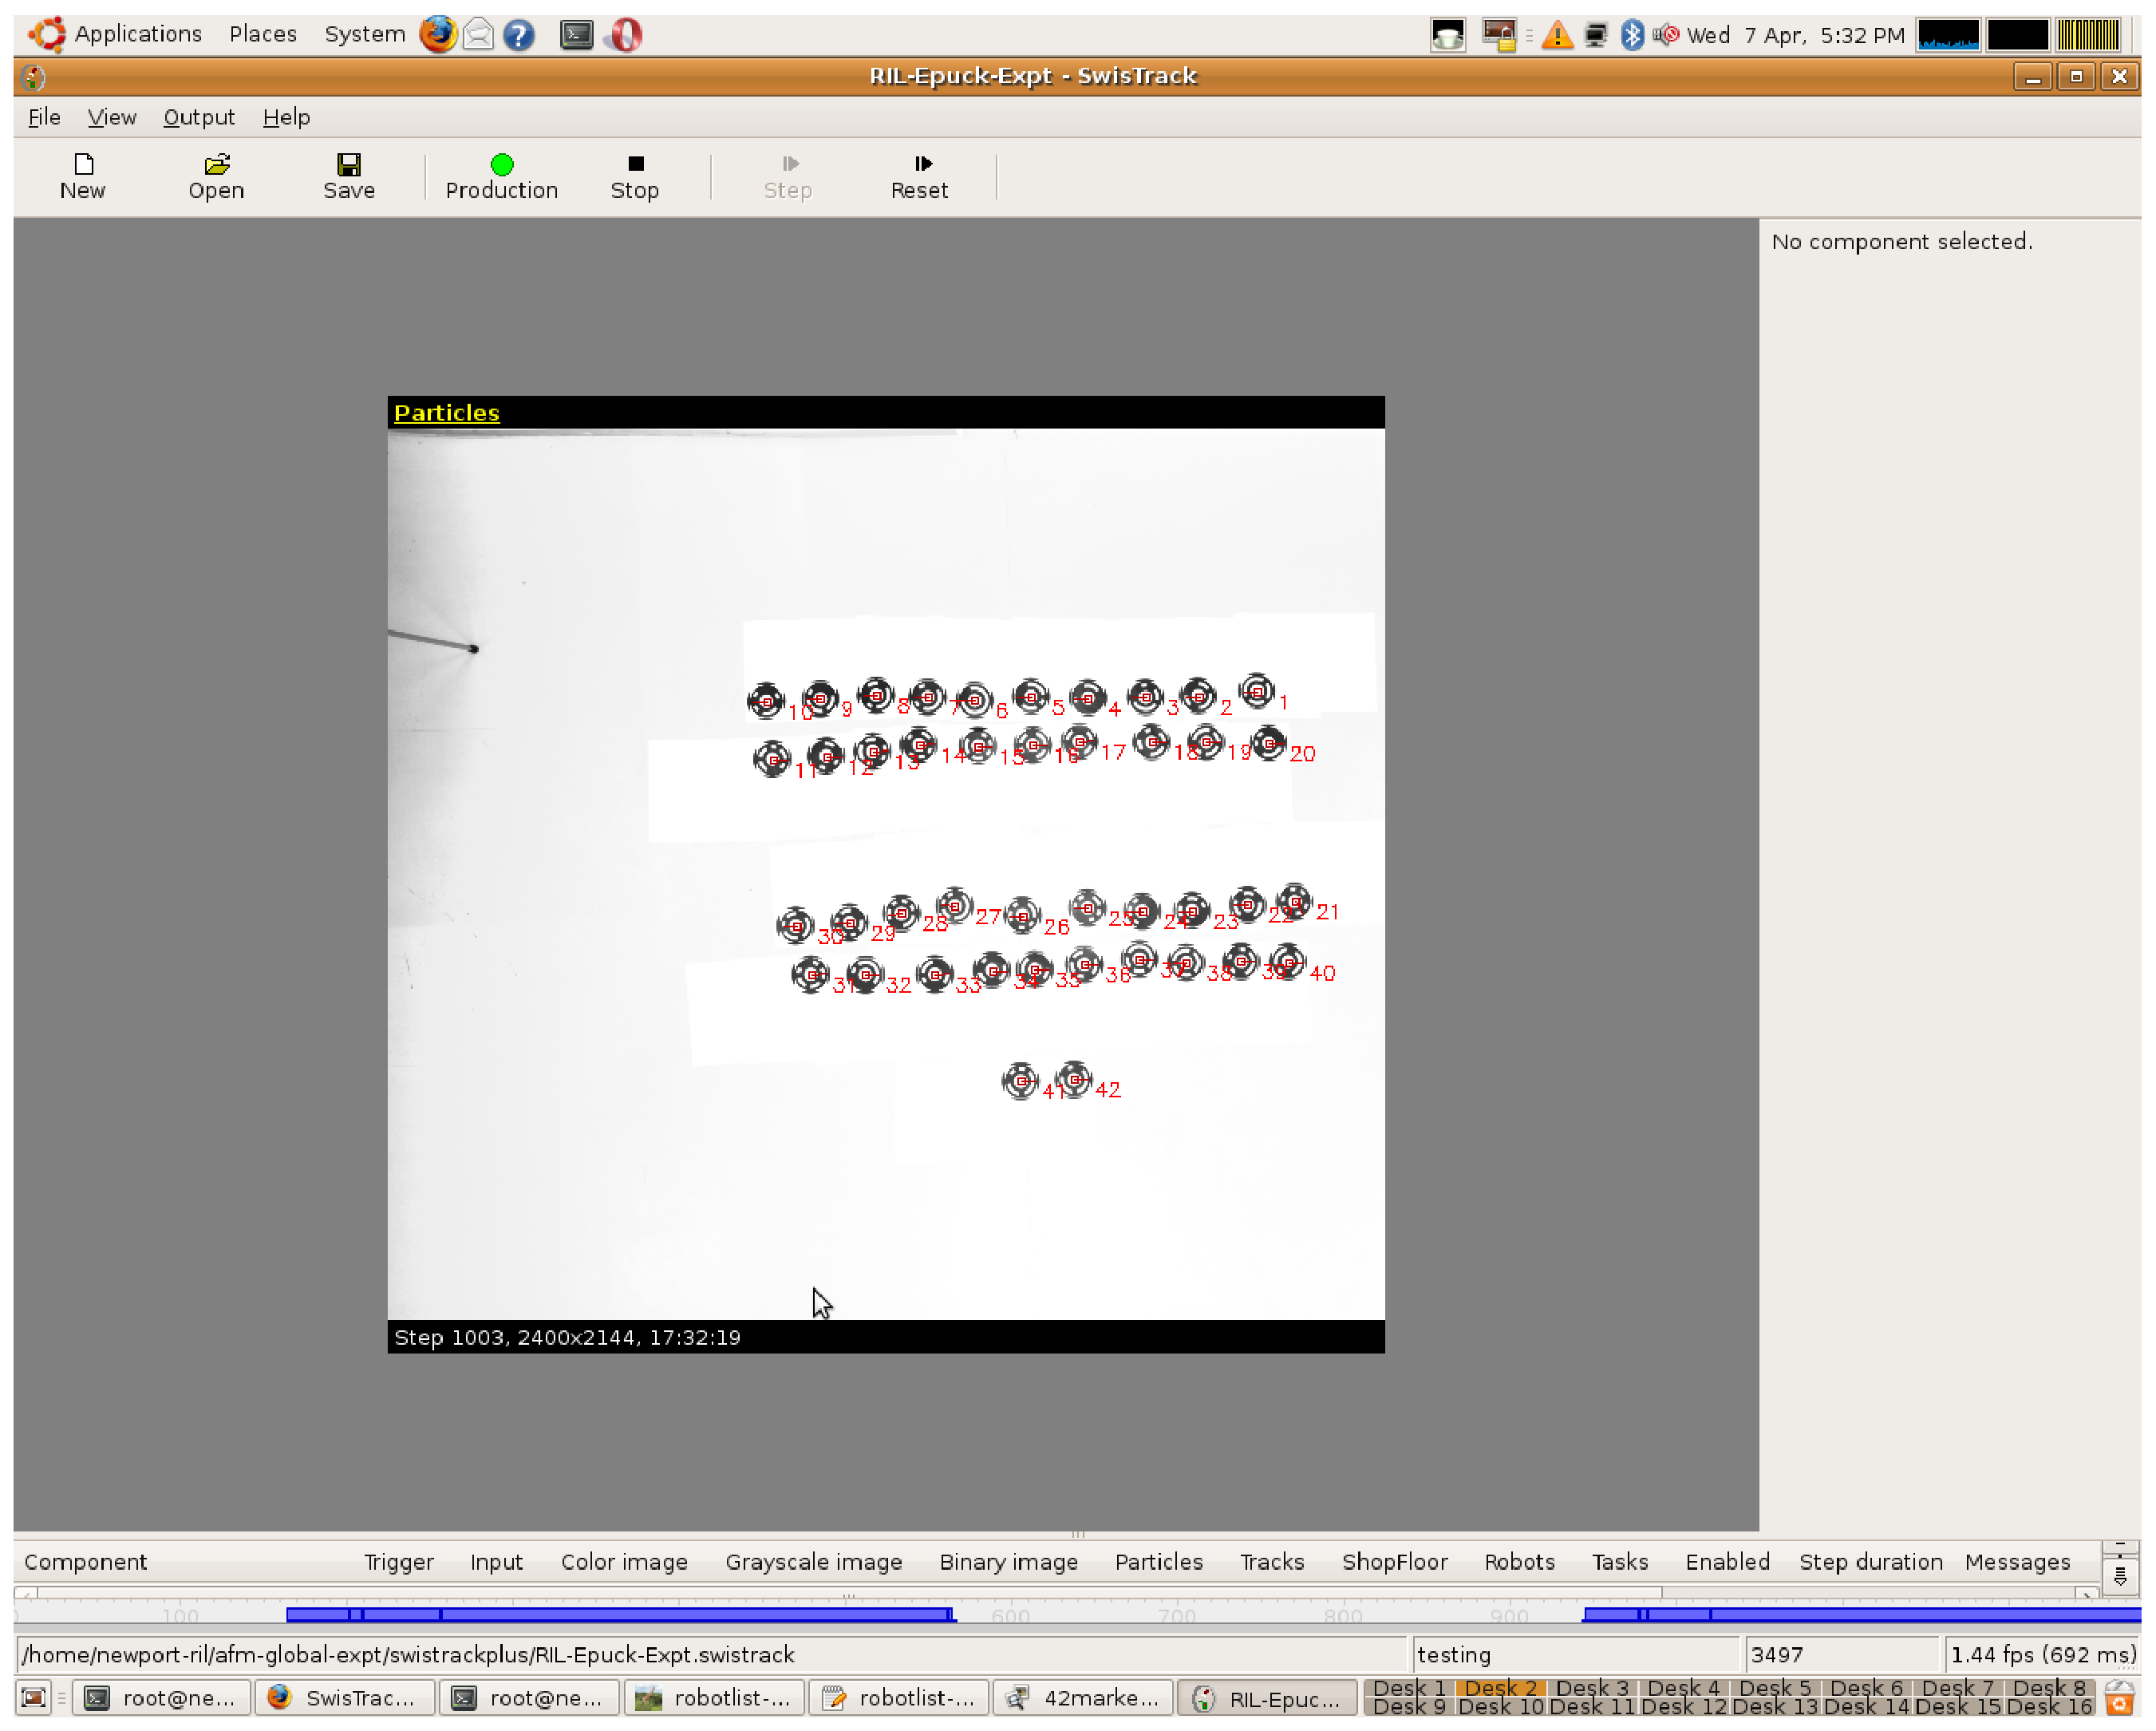
\epsfig{file=Screenshot-42Markers.eps,width=0.8\linewidth,clip=} 
\end{figure}
\end{frame}

\begin{frame}[t]{Conclusion: \alert{our story ends when they start living happily :)}}
 \begin{block}{Journey towards self-regulation }
    \begin{itemize}
    \item Robots can do self-regulation of tasks by \alert{{\em listening} attractive field, concurrency, learning, forgetting}
    \item \alert{Plasticity and task specialization} : DoL observed
    \item Without much dependence on any particular \alert{communication/sensing} paradigm
    \item Now It's the time for \alert{Solving real-world problems}
    \end{itemize}
  \end{block}
\end{frame}

\end{document}


